\documentclass{article}
\usepackage[margin=1.25in]{geometry}
\usepackage{amsmath, amssymb, setspace, enumerate, enumitem}
\usepackage{setspace}
\usepackage{graphicx}
\onehalfspacing

\begin{document}
    \begin{enumerate}
        \item Exercise 2.8
        \begin{enumerate}[label=(\alph*)]
            \item We know that $\overline{g}$ is the average function of many different hypothesis $g_1,\ g_2,...,\ g_n$ of different data sets. $H$ represents the hypotheses set, where each hypothesis in $H$ is dependent on their respective data set. If the hypothesis in $H$ are in linear combination, then the average of the hypotheses in $H$ should also be a linear combination, proving that $\overline{g} \in H \hfill \blacksquare$
            \item We can imagine a model with two hypotheses, one that will label all datapoints as $+1$ and another as $-1$, then the average of those two hypotheses will be $0$, which is not in the hypothesis set, therefore $\overline{g} \notin H \hfill \blacksquare$
            \item (b) is a binary classification and $\overline{g}$ is not a binary function since $0 \notin \{+1, -1\}$. Often, with more hypotheses, the average will be a number between $\{-1, 1\}$, it will be unlikely that they are $+1$ or $-1$
        \end{enumerate}

        \item Problem 2.14
        \begin{enumerate}
            \item Given that the $d_{vc}$ is finite, we know that the hypothesis can shatter any data set of size $d_{vc}$. We can claim that $K(d_{vc}) \geq d_{vc}(H)$, since $K(d_{vc})$ assumes that every $K$ hypothesis can shatter the maximum number of points, $d_{vc}$. Then $K(d_{vc} + 1) > K(d_{vc}) \geq d_{vc}(H)$, by transitivity, $K(d_{vc} + 1) > d_{vc}(H) \hfill \blacksquare$
            \item Given that the hypothesis has a finite VC dimension, then we have a breakpoint such that $2^\ell > \ell^{d_{vc}} + 1$ If we have $K$ hypotheses, then $m_H(\ell) \leq K(\ell^{d_{vc}}+1)$. By inspection, $2K\ell^{d_{vc}} > K(\ell^{d_{vc}} + 1)$. So here we know that $2^\ell > 2K\ell d^{vc} > K(\ell ^{d_{vc}} + 1)$, by transitivity, $2^\ell > K(\ell ^{d_{vc}} + 1)$, which means $2^\ell > m_H(\ell)$, if this is true, then it means that there are no hypothesis can shatter $2^\ell$ points, which means that $d_{vc} \leq \ell \hfill \blacksquare$
            \item \textbf{TO DO}
        \end{enumerate}

        \item Problem 2.15
        \begin{enumerate}
            \item Consider $x_1$ is a point with coordinates $i_1, j_1$, then $h(i_1, j_1) = sign(i_1 + j_1)$. For the purpose of this example, we will consider $x_2 = (i_2, j_2)$, where $h(i_2, j_2) = sign(i_2, j_2)$. If $i_1 > i_2$ and $j_1 > j_2$, then $sign(i_1 + j_1) > sign(i_2 + j_2)$. We can consider the following graph:\\
            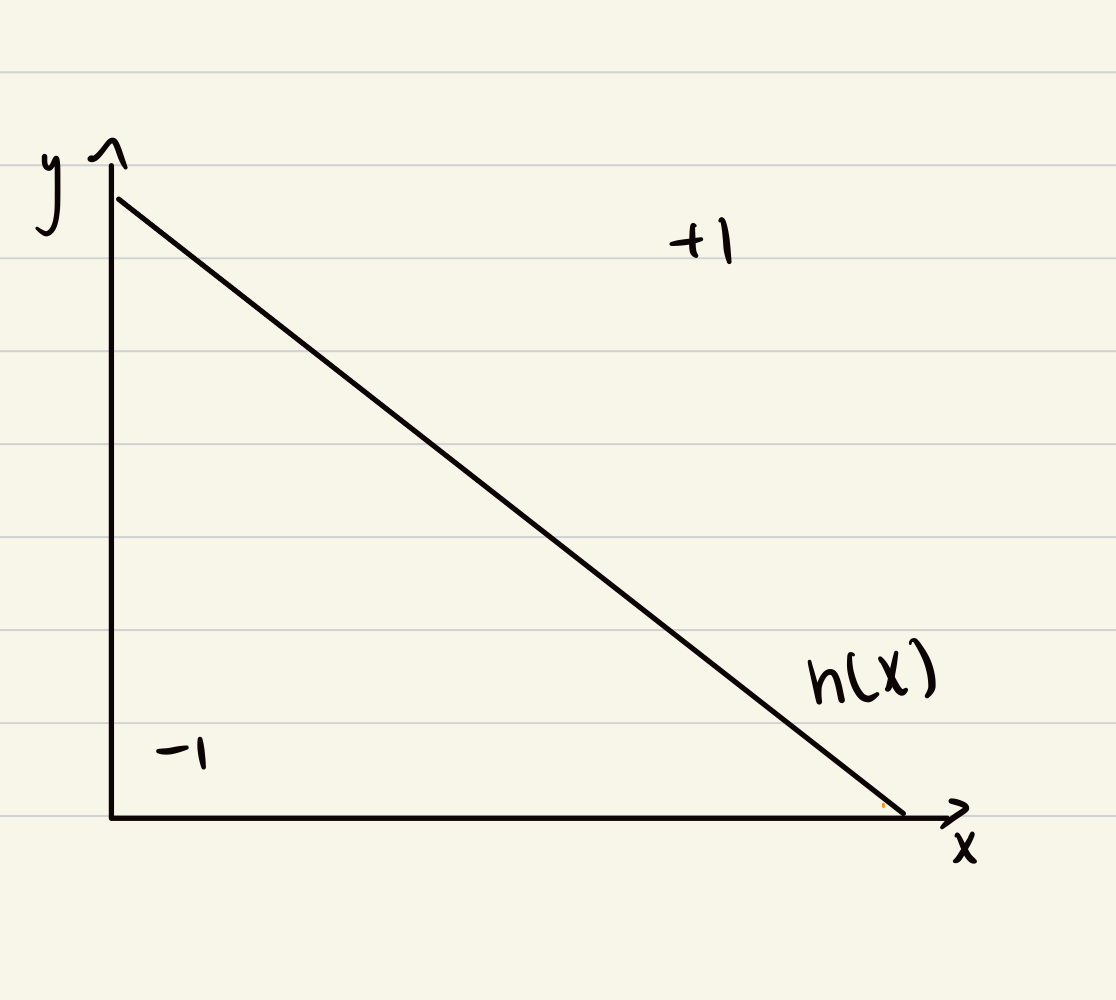
\includegraphics[scale=0.25]{images/2_15_1.png}

            \item If we begin with a point and increase the first component, let that be $i_1$ and decrease the second component, let that be $j_1$, then we will continuously generate the value $sign(i_n, j_n)$ for $\sum_{n = 1}^{N}$. It doesn't matter the number of points that are generated, there will always be a way to represents all the dichotomies, therefore, the maximum number of dichotomies is $m_H(N) = 2^N$, by definition, $d_{VC} = \infty$
        \end{enumerate}

        \item Problem 2.24
        \begin{enumerate}[label=(\alph*)]
            \item We don't know the target function, but out hypothesis set has functions in the form of $ax + b$, so $x^2_1 = ax_1 + b$ and $x^2_2 = ax_2 + b$, with algebra manipulation, we get to $a = x_1 + x_2$ and $b = -x_2x_1$. By definition, we know $\overline{g}(x) = E_D[g^{(D)}(x)] = E_D[(x_1+x_2)x - x_2x_1]$
            \begin{align*}
                    \overline{g}(x) &= x \cdot E[(x_1+x_2-x_2x_1)]\\
                    &= x \cdot E[x_1] + E[x_2] - E[x_2x_1]
            \end{align*}
            By definition, $E[x] = \int^{+1}_{-1}xdx = 0$, given that we have two datapoints, the average $\overline{g}(x) = \frac{1}{2}(x \times 0 + 0 - 0) = 0$
            
            \item Generate a test dataset of size $2N$, then we run $N$ trials, picking two points at a time:
            \begin{itemize}
                \item for $\overline{g}(x)$, generate N trials, each trial contains 2 points, compute $g^D(x) = (x_1 + x_2)x - x_2x_1$, then we can compute the average by $\overline{g}(x) = \frac{1}{N}\sum_{i = 0}^{N}g_i(x)$
                \item we can computer out of sample error by (2.17)
                \begin{align*}
                    E_{out}(g^D) &= E_x[(g^D(x) - f(x))^2]\\
                    &= \int_{-1}^{1}(\frac{1}{N}\sum_{i = 1}^{N}(g_i(x) - f(x))^2)dx
                \end{align*}
                or, if we have bias and var, simply
                \begin{align*}
                    E_D[E_{out}(g^D)] = bias + var
                \end{align*}
                \item we can compute bias by $bias(x) = (\overline{g}(x) - f(x))^2$
                \item we can compute var by $var(x) = E_D[(g^D(x) - \overline{g}(x))^2]$
                \begin{align*}
                    E_D[(g^D(x) - \overline{g}(x))^2] &= \int_{-1}^{1}(\frac{1}{N}\sum_{i = 1}^{N}(g_i(x) - \overline{g}(x))^2)dx
                \end{align*}
            \end{itemize}

            \item ok
        \end{enumerate}
    \end{enumerate}
\end{document}